\Titelbanner{10}{Integralrechnung}

\paragraph{Wiederholung Integralrechnung}$~$

\begin{itemize}
    \item Integrale von Polynomen: $\int \dd{x} (x^3+5x^2+1) = \frac{x^4}{4}+\frac{5x^3}{3} + x + C.$ 
    \item Logarithmische Integration: $\int \dd{x} \frac{2x+3}{x^2+3x+19} = \ln|x^2+3x+19| + C$ 
    \item Integrale mit Wurzeln: $\int \dd{x} \frac{1}{\sqrt{x}} = 2\sqrt{x} + C$
    \item Partielle Integration: $\int\limits_{a}^{b} \dd{x} u'(x) v(x) = u(x) v(x)\eval_a^b - \int\limits_{a}^{b}\dd{x} u(x) v'(x)$
\end{itemize}

\emph{Tafelbeispiel:}
\begin{align}
    \int \dd{x} \underbrace{x^n}_{u'} \underbrace{\ln(x)}_{v} &= \frac{x^{n+1}}{n+1} \ln(x) - \int \dd{x} \frac{x^{n+\cancel{1}}}{n+1}\cdot \frac{1}{x} \quad (n\neq -1) \\
    &= \frac{x^{n+1}}{n+1} - \frac{x^{n+1}}{(n+1)^2} + C= \uuline{\frac{x^{n+1}}{(n+1)^2}((n+1)\ln(x)-1) + C}
\end{align}

\paragraph{Aufgabe 1: } \emph{Stammfunktionen} \hfill Ziel: (a) bis (d)\\[0.2cm]
\emph{Bestimmen Sie jeweils die Stammfunktion $F(x)$ der folgenden Funktionen.}
\emph{Hinweis: Partialbruchzerlegung in (e).}\\[1cm]

\begin{enumerate}[label=(\alph*)]
    \setlength{\mathindent}{0pt}
    \item$~$\\[-1.5cm] 
    \begin{align}
        f(x)=\sin(2x+5) \quad \Rightarrow \quad F(x) = \int \dd{x} \sin(2x+5) = \uuline{-\frac{\cos(2x+5)}{2}+C}.
    \end{align}
    \item$~$\\[-1.5cm]
    \begin{align}
        f(x)=\frac{k}{kx+1} \quad \Rightarrow \quad F(x) = k \int \dd{x} \frac{1}{kx+1} = \uuline{\ln|kx+1| + C}
    \end{align}
    \item$~$\\[-1.5cm] 
    \begin{align}
        f(x)=\frac{\cos(x)}{\sin(x)} \quad \Rightarrow \quad F(x) = \int \dd{x} \frac{\cos(x)}{\sin(x)} = \uuline{\ln(\sin(x))+C}
    \end{align}
    \item $f(x)=\frac{a\cos(x)+b\sin(x)}{c\sin(x)} = \frac{a}{c}\frac{\cos(x)}{\sin(x)} + \frac{b}{c}$
    \begin{align}
        F(x) = \frac{a}{c} \int\dd{x} \frac{\cos(x)}{\sin(x)} + \frac{b}{c} \int \dd{x} = \uuline{\frac{a \ln(\sin(x))+bx}{c}+ C}  
    \end{align}
    \item$~$\\[-1.5cm] 
    \begin{align}
        f(x)=\frac{x^2+1}{x^2-1} &= \alpha + \frac{\beta}{x+1} + \frac{\gamma}{x-1}  \\
        \Rightarrow x^2 + 1 &= \alpha (x^2-1) + \beta (x-1) + \gamma (x+1) = \underbrace{\alpha}_{=1} x^2 + \underbrace{(\beta+\gamma)}_{=0} x + \underbrace{(\gamma - \beta -\alpha)}_{=1} \\[-5mm]
        \frac{x^2+1}{x^2-1} &= 1 - \frac{1}{x+1} + \frac{1}{x-1} \\
        F(x) &= \int\dd{x} - \int\frac{\dd{x}}{x+1} + \int \frac{\dd{x}}{x-1} = \uuline{x + \ln(\frac{x-1}{x+1})+C} 
    \end{align}
    \item$~$\\[-1.5cm]  
    \begin{align}
        f(x)=\frac{kx}{\sqrt{x^2+y^2}^3} \quad \Rightarrow \quad F(x) = k \int \frac{x}{\sqrt{x^2+y^2}^3} \dd{x} = \uuline{- \frac{k}{\sqrt{x^2+y^2}} + C}.
    \end{align}
\end{enumerate}
%
\paragraph{Aufgabe 2: } \emph{Partielle Integration}\hfill Ziel: (a) bis (c)\\[0.2cm]
\emph{Bestimmen Sie die folgenden Integrale unter Verwendung partieller Integration.}

\begin{enumerate}[label=(\alph*)]
    \setlength{\mathindent}{0pt}
    \item$~$\\[-1.7cm]
    \begin{align}
        \int\limits_0^\pi \underbrace{x}_{u}\underbrace{\sin(x)}_{v'}\dd{x} = \qty(-x \cos(x))\eval_0^\pi + \int\limits_{0}^{\pi} \cos(x) \dd{x} = \pi + \sin\eval_0^\pi = \uuline{\pi}
    \end{align}
    \item$~$\\[-1.7cm]
    \begin{align}
        \int\limits_0^1 \underbrace{x^3}_{u}\underbrace{\e^{x}}_{v'}\dd{x} &= x^3 \e^x \eval_0^1 - 3 \int\limits_{0}^{1} x^2 \e^x \dd{x} = \e - 3(x^2 \e^x)\eval_0^1 + 6 \int\limits_{0}^{1}x\e^x \dd{x} \\
        &= -2\e + \cancel{6(x\e^x)\eval_0^1} - 6 \underbrace{\int\limits_{0}^{1}\e^x \dd{x}}_{\cancel{\e}-1} = \uuline{6-2\e}.
    \end{align}
    \item$~$\\[-1.7cm]
    \begin{align}
        \int\limits_{r_0}^{2r_0} \underbrace{r\vphantom{\qty(\frac{1}{1})}}_{u'}\underbrace{\qty(1+\ln \frac{r}{r_0})}_{v} \dd{r} &= \eval[\frac{r^2}{2}\qty(1+\ln \frac{r}{r_0})|_{r_0}^{2r_0} - \frac{1}{2} \int\limits_{r_0}^{2r_0} r^{\cancel{2}} \cdot \frac{1}{\cancel{r}} \dd{r} \\
        &= 2 r_0^2 (1+\ln2) - \frac{r_0^2}{2} - \frac{1}{4}(4r_0^2 -r_0^2) = \uuline{\qty(\frac{3}{4}+2\ln2)r_0^2}
    \end{align}
    \item$~$\\[-1.5cm]
    \begin{align}
        \underbrace{\int \frac{\ln(x)}{x}\dd{x}}_{\mathclap{u'= \frac{1}{x}, v=\ln(x)}} = \ln^2(x) - \int \frac{\ln(x)}{x} \quad \Rightarrow \int \frac{\ln(x)}{x}\dd{x} = \uuline{\frac{\ln^2(x)}{2} + C}.
    \end{align}
\end{enumerate}

\paragraph{Aufgabe 3: } \emph{Substitutionen}\\[0.2cm]
\emph{Berechnen Sie die folgenden Integrale jeweils unter Verwendung der angegebenen Substitution.}

\emph{Tafelbeispiel:}
\begin{align}
    \int \dd{x} \ln(x) &= \int \dd{u} u \e^{(n+1)u} \overset{\text{P.I.}}{=} \frac{u \e^{(n+1)u}}{n+1} - \underbrace{\int \dd{u} \frac{\e^{(n+1)u}}{n+1}}_{\displaystyle\frac{\e^{(n+1)u}}{(n+1)^2}}= \uuline{\frac{x^{n+1} \ln(x)}{n+1} - \frac{x^{n+1}}{(n+1)^2}} \\[-8mm]
    \text{Subst. } u&= \ln(x), \quad \dd{x} = \e^u \dd{u} 
\end{align}
\emph{Lösung:}
\begin{enumerate}[label=(\alph*)]
    \setlength{\mathindent}{0pt}
    \item$~$\\[-1.7cm]
    \begin{align}
        \int\limits_{0}^{1} \sqrt{1-x^2} \dd{x} &= \int\limits_{0}^{\pi/2} \dd{\varphi} \cos(\varphi) \sqrt{1-\sin^2(\varphi)} = \int\limits_{0}^{\pi/2} \dd{\varphi} = \int\limits_{0}^{\pi/2}\dd{\varphi} \frac{1+\cos(2\varphi)}{2} \notag \\
        &\qquad x = \sin\varphi,\quad \dd{x} = \cos\varphi \dd{\varphi}, \qq{Grenzen} x=0: \varphi=0, \quad x=1: \varphi = \frac{\pi}{2} \\
        &= \eval[\frac{\varphi}{2} + \frac{\sin(2\varphi)}{4}|_0^{\pi/2} = \uuline{\frac{\pi}{4}}
    \end{align}
    \item$~$\\[-1.7cm]
    \begin{align}
        \int\limits_0^1 \frac{\dd{x}}{(1+x^2)\sqrt{\arctan(x)}} &= \int\limits_{0}^{\pi/4} \frac{\dd{u}}{\sqrt{u}} = 2 \sqrt{u} \eval_0^{\frac{\pi}{4}} = \uuline{\sqrt{\pi}} \\
        u = \arctan(x), \quad \dd{u} &= \frac{\dd{x}}{1+x^2}, \qq{Grenzen} x=0: u=0, \quad x=1: u=\frac{\pi}{4}
    \end{align}
\end{enumerate}

\paragraph{Aufgabe 4: } \emph{Vollständige Induktion} \hfill (Zusatzaufgabe)\\[0.2cm]
\emph{Zeigen Sie mithilfe vollständiger Induktion, dass für die Fakultät}
\begin{align*}
    n! = \int\limits_{0}^{\infty} x^n \e^{-x} \dd{x},
\end{align*}
\emph{gilt. Hinweis: Es gilt $0! = 1$.}
\begin{enumerate}
    \setlength{\mathindent}{0cm}
    \item[(IA)] $n=0: \quad 0! = \int\limits_{0}^{\infty} \e^{-x} \dd{x} = -\e^{-x}\eval_0^\infty = -(0-1) = 1 \quad\checkmark$ 
    \item[(IV)] $n=k: \quad k! = \int\limits_{0}^{\infty} x^k \e^{-x} \dd{x}$
    \item[(IB)] $n=k+1: \quad (k+1)! = \int\limits_{0}^{\infty} x^{k+1} \e^{-x} \dd{x}$\\
    \begin{proof}$~$\\[-1.8cm]
        \begin{align}
            \hspace{1.5cm} \int\limits_{0}^{\infty} x^{(k+1)} \e^{-x} \dd{x} \overset{\text{P.I.}}{=} \underbrace{\eval(-x^{k+1} \e^{-x}|_0^\infty}_{=0} + (k+1) \underbrace{\int\limits_{0}^{\infty} x^k \e^{-x} \dd{x}}_{k!} = (k+1)k! = (k+1)!
        \end{align}
    \end{proof}
\end{enumerate}

\paragraph{Aufgabe 5: } \emph{Flächenintegral}\\[0.2cm]

\emph{Tafelbeispiel:} Eingeschlossene Fläche einer Parabel $y(x) = 1-x^2$ mit der $x$-Achse. 
\begin{align}
        A = \int\limits_{-1}^{1} \dd{x} \int\limits_{0}^{y(x)}\dd{y} = \int\limits_{-1}^{1}\dd{x} \int\limits_{0}^{1-x^2} \dd{y} = \int\limits_{-1}^{1}\dd{x} (1-x^2) = \eval(x-\frac{x^3}{3}|_{-1}^1 = \frac{4}{3}.
\end{align}
\emph{Leiten Sie die Formel für den Flächeninhalt eines Kreises vom Radius $R$ her.}
\begin{center}
    \begin{tikzpicture}[scale=0.6]
        \draw[-{latex}, line width=1pt] (0,-3.5)--(0,3.5);
        \draw[-{latex}, line width=1pt] (-3.5,0)--(3.5,0);
        \draw (0,0) circle (80pt);
        \node at (0,3.7) {$y$};
        \node at (3.7,0) {$x$};
        \draw[line width=0.5pt] (2.05,2.05)--(2.5,2.5);
        \draw[line width=0.5pt] (2.05,-2.05)--(2.5,-2.5);
        \node at (3.4,2.85) {$y=\sqrt{R^2-x^2}$};
        \node at (3.4,-2.8) {$y=-\sqrt{R^2-x^2}$};
        \draw[->,line width=0.5pt] (0,0)--(-2,1.98);
        \node at (-0.9,1.3) {$R$};
    \end{tikzpicture}
\end{center}
\vspace{-1cm}
\begin{align}
    \frac{A}{4} &= \int\limits_{0}^{R} \dd{x} \int\limits_{0}^{\sqrt{R^2-x^2}}\dd{y} = \int\limits_{0}^{R} \dd{x} \sqrt{R^2-x^2} = R \int\limits_{0}^{R}\dd{x} \sqrt{1-\frac{x^2}{R^2}} \qq{Subst.} z = \frac{x}{R} \\
    &= R^2 \int\limits_{0}^{1} \dd{z} \sqrt{1-z^2} \overset{(3a)}{=} \frac{\pi R^2}{4} \quad \Rightarrow \uuline{A = \pi R^2}
\end{align}
% \vspace{1cm}
%
\paragraph{Aufgabe 6: } \emph{Volumenintegral} \hfill (Zusatzaufgabe)\\[0.2cm]
\emph{Berechnen Sie das Volumen des in der Abbildung gezeigten Körpers.}
% \begin{center}
% 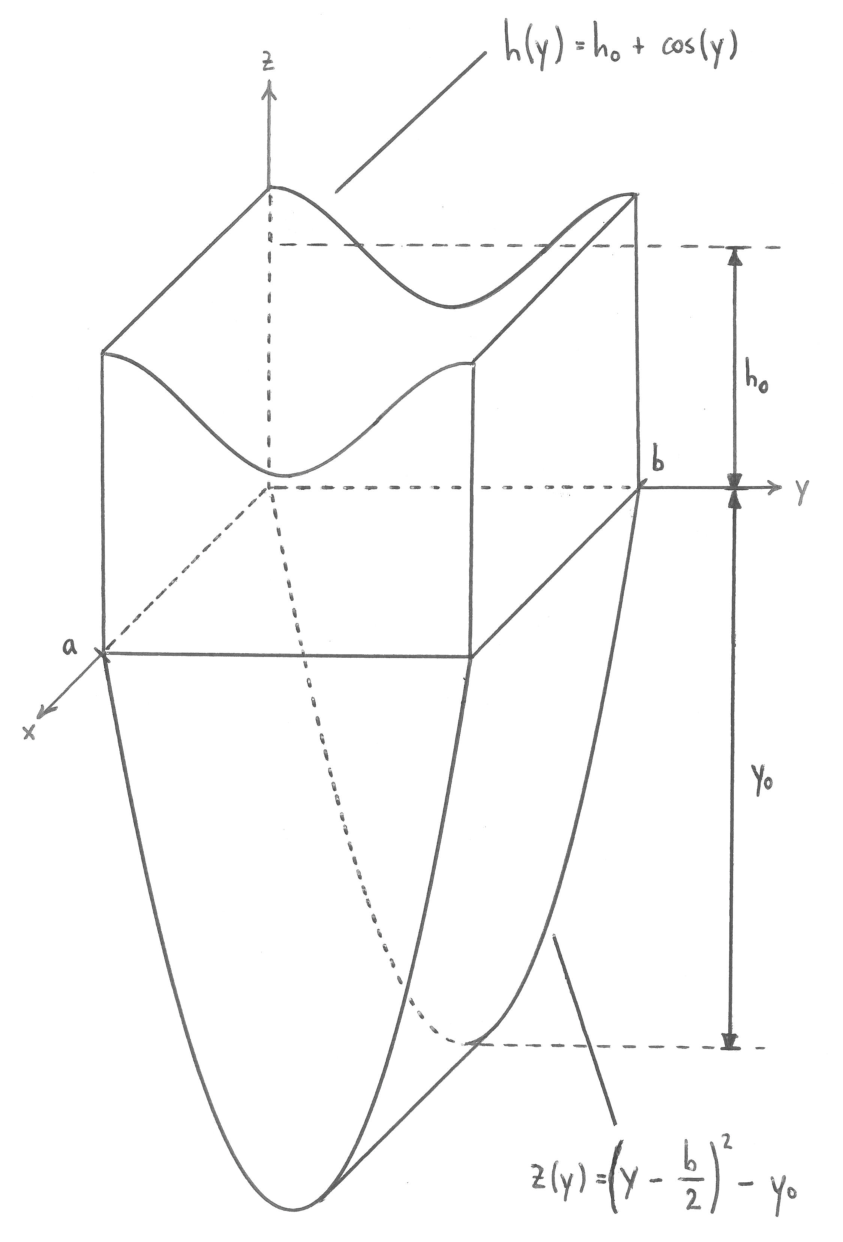
\includegraphics[width=8cm]{koerper.pdf}
% \end{center}

\begin{figure}[htp]
    \centering
    \begin{tikzpicture}[scale=0.7]
        \draw[dashed] (0,0) -- (-1.4,-1.4);
        \draw[dashed] (0,0) -- (0,2.4);
        \draw[dashed] (0,0) -- (4,0);
        \draw[thick,-{latex}] (-1.4,-1.4) -- +(-0.707,-0.707)node[below]{$x$};
        \draw[thick,-{latex}] (4,0) -- +(2,0)node[right]{$y$};
        \draw[thick,-{latex}] (0,2.4) -- +(0,1)node[above]{$z$};
        \draw[thick] (2+0.25,-6+0.0625) -- +(-1.4,-1.4);
        \draw[thick] (-1.4,-1.4) -- ++(4,0) -- ++(1.4,1.4);
        \draw[dashed] (0,1.9) -- +(5.5,0);
        \draw[dashed] (2,-6) -- +(3.5,0);
        \draw[thick, {latex}-{latex}] (5,1.9) --node[right]{$h_0$} (5,0);
        \draw[thick, {latex}-{latex}] (5,0) --node[right]{$y_0$} (5,-6);
        \node (A) at (-1.4-.25,-1.38){$a$};
        \node (A) at (4.2,0.2){$b$};
        \draw[ domain=2:4, smooth, variable=\x] plot ({\x}, {1.5*(\x-2)*(\x-2)-6});
        \draw[ domain=0:2, dashed, smooth, variable=\x] plot ({\x}, {1.5*(\x-2)*(\x-2)-6});
        \draw[ domain=-1.4:2.6, smooth, variable=\x] plot ({\x}, {1.5*(\x-0.6)*(\x-0.6)-6-1.4});
        \draw[ domain=-1.4:2.6, smooth, variable=\x] plot ({\x}, {0.5*cos(deg((\x+1.4)*3.1415/2))+0.5});
        \draw[ domain=0:4, smooth, variable=\x] plot ({\x}, {0.5*cos(deg((\x)*3.1415/2))+0.5+1.4});
        \draw[thick] (-1.4,-1.4) -- ++(0,2.4) -- ++(1.4,1.4);
        \draw[thick] (2.6,-1.4) -- ++(0,2.4) -- ++(1.4,1.4) -- ++(0,-2.4);
        \node[anchor=west] at (0.7,2.9){$h(y)=h_0 + \cos(y) $};
        \draw[thick, -{latex}] (1.1,2.6) --+(-0.4,-.4);
        \node[anchor=west] at (2,-7){$z(y) = \qty(y-\frac{b}{2})^2 - y_0 $};
        \draw[thick, -{latex}] (3,-6.6) --+(-.2,1.3);
    \end{tikzpicture}
\end{figure}

\begin{align}
    V = \int\limits_{0}^{a}\dd{x} \int\limits_{0}^{b}\dd{y} \int\limits_{\qty(y-\frac{b}{2})^2 - y_0}^{h_0 + \cos(y)} \dd{z} &= a \int\limits_{0}^{b} \dd{y} (h_0 + \cos(y) - y^2 - \frac{b^2}{4} + by + y_0) \\
&= ab\qty(h_0 + y_0 - \frac{b^2}{4}) + a \underbrace{\int\limits_{0}^{b}\dd{y} (\cos(y)-y^2 + by)}_{\displaystyle \Bigg(\sin(y) - \frac{y^3}{3} + \frac{by^2}{2}\eval_0^b} \\
&= \uuline{ab\qty(h_0 + y_0 - \frac{b^2}{12})+ a\sin(b)}
\end{align}